
\documentclass[11pt, conference, onecolumn]{IEEEtran} 
% IEEE INFOCOM 
%\documentclass[10pt, conference, letterpaper]{IEEEtran}

% the default nsl packages
\usepackage{epsfig}
\usepackage{times}
\usepackage{subcaption}
\usepackage{amsfonts}
\usepackage{amsmath}
\usepackage{amssymb}
\usepackage{graphicx}
\usepackage{url}
\usepackage{psfrag}
\usepackage{array}
\usepackage{mdwmath} % part of Mark Wooding's powerful
\usepackage{mdwtab}  % tools for math, tables, ...
\usepackage{multirow}
\usepackage{verbatim}
\usepackage{color}


% added packages
\usepackage{paralist} % for inparaenum
\usepackage{algorithm}% http://ctan.org/pkg/algorithms
\usepackage{algpseudocode}
\usepackage{xspace} % using space in newcommand
\usepackage{cleveref} % multi-label ref


\catcode`"=\active
\gdef"#1"{{\sf #1}}

\newcommand{\handout}[2]{
University of Texas at Austin\hfill{#2}
\newline
Department of Computer Science
\newline
Probabilistic Methods, Spring 1992
\newline
Handout \##1
\newline
}

\newcommand{\lecture}[4]{
University of Texas at Austin\hfill{#2}
\newline
Department of Computer Science
\newline
Probabilistic Methods, Spring 1992\hfill Lecturer: {#3}
\newline
Lecture \##1\hfill Scribe: {#4}
\newline
}

%\setlength{\parskip}{0.85ex}
%\setlength{\parindent}{0pt}

\newcommand{\id}[1]{{\it #1}}

\newcommand{\Eqnum}[1]{(\ref{eqn:#1})}
\newcommand{\Eqn}[1]{Equation~\Eqnum{#1}}
\newtheorem{Convention}{Convention}
\newtheorem{Definition}{Definition}
\newtheorem{Theorem}{Theorem}
\newtheorem{Example}{Example}[section]
\newtheorem{Remark}{Remark}
\newtheorem{Notation}{Notation}
\newtheorem{F}{Fact}
\newtheorem{Lemma}{Lemma}
\newtheorem{Corol}{Corollary}[Theorem]
\newtheorem{Lcorol}{Corollary}[Lemma]
\newtheorem{Proposition}{Proposition}

%\newenvironment{Proof}{\noindent{\bf Proof: }}{\hfill$\Box$}
\newenvironment{Invariant}[1]{\begin{quote}{Invariant\em#1\/}:}{\end{quote}}
%\newenvironment{Convention}[1]{\begin{quote}{Convention\em#1\/}:}{\end{quote}}
%\newcommand{\qed}{\protect\raisebox{.3ex}{\framebox[.5em]{\rule{0em}{.6ex}}}}

%\newcommand{\qed}{\nobreak \ifvmode \relax \else
%\ifdim\lastskip<1.5em \hskip-\lastskip
%\hskip1.5em plus0em minus0.5em \fi \nobreak
%\vrule height0.75em width0.5em depth0.25em\fi}

%%%% another environment for proof
%\newenvironment{proof}[1][Proof]{\begin{trivlist}
%\item[\hskip \labelsep {\bfseries #1}]}{\end{trivlist}}
%\newenvironment{definition}[1][Definition]{\begin{trivlist}
%\item[\hskip \labelsep {\bfseries #1}]}{\end{trivlist}}
%\newenvironment{example}[1][Example]{\begin{trivlist}
%\item[\hskip \labelsep {\bfseries #1}]}{\end{trivlist}}
%\newenvironment{remark}[1][Remark]{\begin{trivlist}
%\item[\hskip \labelsep {\bfseries #1}]}{\end{trivlist}}


\newcommand{\equals}{\stackrel{\rm def}{=}}
\newcommand{\ceil}[1]{\left\lceil  #1 \right\rceil}
\newcommand{\floor}[1]{\left\lfloor  #1 \right\rfloor}

\newcommand{\bin}[2]{\mathop{\mbox{\rm bin}}(#1,#2)}
\newcommand{\smallbin}[2]{\mathop{\mbox{\scriptsize{\rm bin}}}(#1,#2)}
\newcommand{\expectation}[1]{\mathop{\mbox{\rm E}}(#1)}
\newcommand{\variance}[1]{\mathop{\mbox{\rm Var}}(#1)}
\newcommand{\covariance}[2]{\mathop{\mbox{\rm Cov}}(#1,#2)}

\newcommand{\polyTime}{{\bf P }}
\newcommand{\NP}{{\bf NP }}
\newcommand{\coNP}{{\bf co-NP }}
\newcommand{\PSPACE}{{\bf PSPACE }}
\newcommand{\RNC}{{\bf RNC }}
\newcommand{\R}{{\bf R }}
\newcommand{\RP}{{\bf RP }}
\newcommand{\coR}{{\bf co-R }}
\newcommand{\coRP}{{\bf co-RP }}
\newcommand{\ZPP}{{\bf ZPP }}
\newcommand{\BPP}{{\bf BPP }}
\newcommand{\PP}{{\bf PP }}

\newcommand{\Iff}{\leftrightarrow}
\newcommand{\IFF}{\Longleftrightarrow}
\newcommand{\imp}{\rightarrow}
\newcommand{\Imp}{\Rightarrow}
\newcommand{\IMP}{\Longrightarrow}

\newcommand{\ints}{{\bf Z}}
\newcommand{\nats}{{\bf N}}
\newcommand{\reals}{{\bf R}}
\newcommand{\nTuples}{\ints^n}


%\renewcommand{\algorithmiccomment}[1]{/* #1 */}
%\renewcommand{\algorithmicloop}{\textbf{begin}}
%\renewcommand{\algorithmicendloop}{\textbf{end}}

\def\>{\hspace{0.27cm}}
%\def\>{\hspace{0.3cm}}
%\def\>{\hspace{0.5cm}}
%\def\^{\vspace{-0.5cm}}
\newcommand{\seprule}{\centerline{\rule{\linewidth}{0.3pt}\vspace{.1in}}}
\newcommand{\seprulelast}{\vspace{-0.1in}\centerline{\rule{\linewidth}{0.3pt}\vspace{-0.1in}}}


\newcommand{\Algorithm}[1]{\bigskip\noindent{\bf Algorithm }
        {#1}\vspace{-2mm}\par\nobreak}
\newcommand{\Protocol}[1]{\bigskip\noindent{}
        {\large \sf \bf {#1}}\vspace{.25cm}\par\nobreak}

\def\bs{\boldsymbol}

\def\bbegin{{\bf begin }} 
\def\bbreak{{\bf break}} 
\def\bfor{{\bf for }} 
\def\bstep{{\bf step }}
\def\bdo{{\bf do }}
\def\bgoto{{\bf goto }}
\def\bif{{\bf if }} 
\def\bfi{{\bf fi}}
\def\bthen{{\bf then }} 
\def\belse{{\bf else }}
\def\belsif{{\bf elsif }}
\def\belif{{\bf elif }}
\def\belseif{{\bf elif }}
\def\bboolean{{\bf boolean }}
\def\bwhile{{\bf while }}
\def\bendwhile{{\bf end while}}
\def\brepeat{{\bf repeat }}
\def\btimes{{\bf times}}
\def\buntil{{\bf until }}
\def\bend{{\bf end }} 
\def\bendif{{\bf end if }} 
\def\band{{\bf and }} 
\def\bor{{\bf or }} 
\def\bcor{{\bf cor }} 
\def\bcand{{\bf cand }} 
\def\bco{{\bf co }} 
\def\boc{{\bf oc}} 
\def\bod{{\bf od}}
\def\bto{{\bf to }}
\def\bdownto{{\bf downto }}
\def\balgorithm{{\bf algorithm }}
\def\bprocedure{{\bf procedure }}
\def\bfunction{{\bf function }}
\def\bint{{\bf int }}
\def\bloop{{\bf loop}}
\def\bexitwhen{{\bf exit when }}
\def\btrue{{\bf true}}
\def\bfalse{{\bf false}}
\def\bassert{{\bf assert }}
\def\breturn{{\bf return }}
\def\bbreak{{\bf break}}
\def\bcase{{\bf case}}
\def\bat{{\bf at }}
\def\bnil{{\bf nil }}
\def\bnull{{\bf null }}
\def\bnot{{\bf not }}
\def\bvar{{\bf var }}
\def\blet{{\bf let }}
\def\bendfor{{\bf endfor }}
\def\bforeach{{\bf foreach }}
\def\define{\stackrel{\rm def}{=}}
\def\bswitch{{\bf swicth }}

\def\cbbegin{\color{magenta} begin \color{black}} 
\def\cbfor{\color{magenta} for \color{black}} 
\def\cbstep{\color{magenta} step \color{black}}
\def\cbdo{\color{magenta} do \color{black}}
\def\cbif{\color{magenta} if \color{black}} 
\def\cbfi{\color{magenta} fi\color{black}}
\def\cbthen{\color{magenta} then \color{black}} 
\def\cbelse{\color{magenta} else \color{black}}
\def\cbelsif{\color{magenta} elsif \color{black}}
\def\cbwhile{\color{magenta} while \color{black}}
\def\cbendwhile{\color{magenta} end while\color{black}}
\def\cbrepeat{\color{magenta} repeat \color{black}}
\def\cbtimes{\color{magenta} times\color{black}}
\def\cbuntil{\color{magenta} until \color{black}}
\def\cbend{\color{magenta} end \color{black}} 
\def\cband{\color{magenta} and \color{black}} 
\def\cbor{\color{magenta} or \color{black}} 
\def\cbcor{\color{magenta} cor \color{black}} 
\def\cbcand{\color{magenta} cand \color{black}} 
\def\cbco{\color{magenta} co \color{black}} 
\def\cboc{\color{magenta} oc\color{black}} 
\def\cbod{\color{magenta} od\color{black}}
\def\cbto{\color{magenta} to \color{black}}
\def\cbdownto{\color{magenta} downto \color{black}}
\def\cbalgorithm{\color{magenta} algorithm \color{black}}
\def\cbprocedure{\color{magenta} procedure \color{black}}
\def\cbfunction{\color{magenta} function \color{black}}
\def\cbloop{\color{magenta} loop\color{black}}
\def\cbexitwhen{\color{magenta} exit when \color{black}}
\def\cbtrue{\color{magenta} true\color{black}}
\def\cbfalse{\color{magenta} false\color{black}}
\def\cbassert{\color{magenta} assert \color{black}}
\def\cbreturn{\color{magenta} return\color{black}}
\def\cbat{\color{magenta} at \color{black}}
\def\cbnil{\color{magenta} nil\color{black}}
\def\cbnull{\color{magenta} null\color{black}}
\def\cbnot{\color{magenta} not \color{black}}
\def\cbvar{\color{magenta} var \color{black}}

\newcounter{leftindent}
%\newenvironment{program}{\setcounter{leftindent}{0}\begin{tabbing}\hspace{15ex}\=\hspace{25em}\=\kill\>}{\end{tabbing}}
\newcommand{\inc}[1]{\addtocounter{leftindent}{#1}\\\>\hspace{\value{leftindent}em}}

\newcommand{\ul}[1]{\underline{#1}}                                             
\newcommand{\fp}[2]{{\bf #1} {\it #2}}
\newcommand{\ty}[1]{{\bf #1}}
\newcommand{\act}[1]{{\sf #1}}
\newcommand{\cur}[1]{{\em #1}}
\newcommand{\nm}[1]{{\tt #1}}
\newcommand{\p}[1]{{\it #1}}
\newcommand{\val}[1]{{\bf #1}\hspace{1.5in}}
\newcommand{\rval}[2]{\begin{minipage}[t]{1.5in}{{\bf #1}}\end{minipage} \
         \begin{minipage}[t]{4.5in}{#2}\end{minipage}
         \vspace{1.5mm}\newline}                  
\newcommand{\struct}[2]{\noindent\hspace*{.5in}
   {\bf struct #1} \{ \newline #2 
   \hspace*{.5in}\}\newline}
\newcommand{\typedef}[2]{\noindent\hspace*{.5in}
   \nm{typedef struct} \{ \newline #2 
   \hspace*{.5in}\} #1;\newline}
\newcommand{\mem}[3]{\hspace*{1in}\makebox[1.2in][l]{\nm{#1}}
   \makebox[1in][l]{\nm{#2}};  /* \nm{#3} */
   \newline}
%\newcommand{\tab}[1]{\noindent\hspace*{.5in}#1\newline}
\newcommand{\xtab}[3]{\begin{minipage}[t]{1in}{#1}\end{minipage} \
                 \begin{minipage}[t]{2in}{#2}\end{minipage} \
                 \begin{minipage}[t]{3.75in}{#3}\end{minipage}
               \vspace{0.05mm}\newline}
\newcommand{\xtabs}[3]{\begin{minipage}[t]{0.4in}{#1}\end{minipage} \
                 \begin{minipage}[t]{0.5in}{#2}\end{minipage} \
                 \begin{minipage}[t]{2.1in}{#3}\end{minipage}
               \vspace{0.05mm}\newline}
\newcommand{\xtabl}[3]{\begin{minipage}[t]{0.5in}{#1}\end{minipage} \
                 \begin{minipage}[t]{0.65in}{#2}\end{minipage} \
                 \begin{minipage}[t]{4.3in}{#3}\end{minipage}
               \vspace*{3mm}\newline}

\newcommand{\twofigs}[2]{\begin{minipage}[t]{3.2in}{#1}\end{minipage} \
          \begin{minipage}[t]{3.2in}{#2}\end{minipage}
          \vspace{1.5mm}\newline}
%2.0in
\newcommand{\twoinch}[1]{\begin{minipage}[t]{1.275in}{#1}\end{minipage}}
%3.3in
\newcommand{\threeinch}[1]{\begin{minipage}[t]{2.6in}{#1}\end{minipage}}
\newcommand{\ltwoinch}[1]{\begin{minipage}[t]{2.0in}{#1}\end{minipage}}
\newcommand{\lthreeinch}[1]{\begin{minipage}[t]{3.3in}{#1}\end{minipage}}


% redefinition of captions
\long\def\@makecaption#1#2{
 \vskip 4pt 
 \@tempdima\hsize
  \advance\@tempdima -1cm
 \setbox\@tempboxa\hbox{\helvix #1: #2}
 \ifdim \wd\@tempboxa >\@tempdima
     {\advance\leftskip .5cm \advance\rightskip .5cm\helvix\baselineskip -2pt #1: #2\par} % SKF: added baselineskip 
  \else
     {\centering \hbox to\@tempdima{\hfil\box\@tempboxa\hfil}}
 \fi}

\DeclareMathOperator*{\argmax}{argmax}
\DeclareMathOperator*{\argmin}{argmin}
\DeclareMathOperator*{\lcm}{lcm}


   % some pre-defined macros, originally from nsl
% symbols
\newcommand{\BigZ}{\ensuremath{\mathcal{Z}}}
\newcommand{\BigV}{\ensuremath{\mathcal{V}}}
\newcommand{\BigS}{\ensuremath{\mathcal{S}}}
\newcommand{\BigM}{\ensuremath{\mathcal{M}}}
\newcommand{\BigP}{\ensuremath{\mathcal{P}}}
\newcommand{\BigD}{\ensuremath{\mathcal{D}}}

% General
\newcommand{\MyComment}[1]{{\bf COMMENT: #1}}
\newcommand{\MyTodo}[1]{{\bf TODO: #1}}
\newcommand{\MyNotice}[1]{{\textcolor{red} {#1}}}

\newtheorem{thm}{Theorem}
\newtheorem{cor}[thm]{Corollary}
\newtheorem{lem}[thm]{Lemma}
\newtheorem{dfn}{Definition}
\newtheorem{pbm}{Problem}
\newtheorem{claim}{Claim}

% add a new command following this template, \xspace for automatic spacing after the macro
% \newcommand{\MacroName}{MacroValue\xspace} 

   % some definitions
\errorcontextlines\maxdimen

% begin vertical rule patch for algorithmicx (http://tex.stackexchange.com/questions/144840/vertical-loop-block-lines-in-algorithmicx-with-noend-option)
\makeatletter
% start with some helper code
% This is the vertical rule that is inserted
\newcommand*{\algrule}[1][\algorithmicindent]{\makebox[#1][l]{\hspace*{.5em}\vrule height .75\baselineskip depth .25\baselineskip}}%

\newcount\ALG@printindent@tempcnta
\def\ALG@printindent{%
    \ifnum \theALG@nested>0% is there anything to print
        \ifx\ALG@text\ALG@x@notext% is this an end group without any text?
            % do nothing
            \addvspace{-3pt}% FUDGE for cases where no text is shown, to make the rules line up
        \else
            \unskip
            % draw a rule for each indent level
            \ALG@printindent@tempcnta=1
            \loop
                \algrule[\csname ALG@ind@\the\ALG@printindent@tempcnta\endcsname]%
                \advance \ALG@printindent@tempcnta 1
            \ifnum \ALG@printindent@tempcnta<\numexpr\theALG@nested+1\relax% can't do <=, so add one to RHS and use < instead
            \repeat
        \fi
    \fi
    }%
\usepackage{etoolbox}
% the following line injects our new indent handling code in place of the default spacing
\patchcmd{\ALG@doentity}{\noindent\hskip\ALG@tlm}{\ALG@printindent}{}{\errmessage{failed to patch}}
\makeatother
% end vertical rule patch for algorithmicx % adds vertical line to algorithmic environment, comment this line if the vertical lines are not required

% rename the algorithms Ensure and Require to Input and Output
\renewcommand{\algorithmicrequire}{\textbf{Input:}}
\renewcommand{\algorithmicensure}{\textbf{Output:}}

\graphicspath{{figs/}}

\begin{document}
\title{TrusTem: Recommendation in Disjoint Trust Networks}

\author{\IEEEauthorblockN{Syed Tanveer Jishan}
\IEEEauthorblockA{Presentation ID 9\\
Student ID 301279717\\
sjishan@sfu.ca}
\and
\IEEEauthorblockN{ Khaled Diab}
\IEEEauthorblockA{Presentation ID 5\\
Student ID 301235653\\
kdiab@sfu.ca}
}

\maketitle

\begin{abstract}
Collaborative filtering (CF) based recommender systems suggest items to users by employing a similarity metric. With the introduction of online social networks, graph-based approach of recommendation has emerged. This approach assumes trust among users and recommends items based on trust. Although it solves cold start problem in recommendation system, user-item coverage decreases. We argue that one of the causes of coverage issue is the disjointedness of trust network, therefore, an item not rated by anyone in a subgraph cannot be recommended to any user in that subgraph. To solve this problem, we propose TrusTem: a recommendation algorithm that merges user-item and trust domains. We have conducted experiments on real-life dataset and compared TrusTem against state-of-art algorithms. Our experiments demonstrate that TrusTem covers $99.8\%$ of user-item pairs, at cost of reducing accuracy up to $8\%$. However, we show numerically that TrusTem does better coverage-accuracy trade-off than these algorithms.
\end{abstract}

\section{Introduction} \label{sec:intro}
Personalized recommender systems predict items ratings to users based on their items preferences. With the increase in popularity of online social networks, the trust-based approach to recommendation has emerged~\cite{Massa:2007,Golbeck:2005,Jamali:2009,Jamali:2010}. In such approach, the friendship/trust network among users is taken into consideration to make recommendations. Trust information can be exploited to get rid of cold start problem, since it is assumed by the sociologists that friends (or people you trust) will have similar attributes, hence similar preferences~\cite{Friedkin:1998}. However, recommending items that are only rated by direct trusted users can lead to item coverage issue. To put it simply, the items a target user may like but not rated by his friends will not be recommended. Therefore, recommender systems take advantage of the transitive property of the trust~\cite{Andersen:2008}, and use trust propagation metrics to estimate trust between indirect neighbors so that more items can be covered for recommendation. 

We argue that despite propagating trust in the trust network, there are still hindrance in the coverage of the items to be recommended, since trust networks are usually a set of \textit{disjoint} subgraphs rather than one large fully connected graph. To verify this claim, we looked into several real life datasets. For instance, we have collected trust information among $7,073$ users in Epinions.com and found that it consists of $17$ disjoint subgraphs. Clearly, trust cannot be propagated from one such subgraph to another, since there exist no edges to connect them. In such cases, if an item is not rated by any of the users within a subgraph, then it cannot be recommended to the target user belonging to that subgraph. Therefore, the issue of item coverage will persist.

In order to propagate trust among these disjoint subgraphs, we propose a new recommender algorithm: TrusTem. TrusTem takes advantage of the transitive property of matrix factorization technique~\cite{Koren:2009}. It considers trust to be in the same domain as the item ratings which results in a hybrid trust based recommender system. In such hybrid recommender system, trust propagation and ratings prediction happen simultaneously. We list the contributions of this report as follows:
\begin{itemize}
\item We define a new research problem in trust-based recommendation system. That is, recommendation in disjoint trust networks.
\item We propose a new solution (TrusTem). Our solution model is based on the idea of merging the rating and trust domains.
\item We evaluate TrusTem using real dataset against stat-of-art trust-based recommendation algorithms. We show that TrusTem covers $99.8\%$ of user-item pairs, at cost of reducing accuracy up to $8\%$.
\end{itemize}

The report is structured as follows. Section 2 surveys trust-based recommenders systems. Section 3 defines the problem of recommendation in disjoint trust networks. Section 4 describes our solution model. We evaluate TruTem in Section 5, before concluding the report in Section 6.


\section{Related Work} \label{sec:related}
MoleTrust~\cite{Massa:2007} considers rating information up to certain depth threshold. In order to propagate trust, a backward exploration is performed. It means that the trust value from user A to user B is the aggregation of trust values between the user A and every other users who directly trust B. Similar to MoleTrust, TidalTrust~\cite{Golbeck:2005} performs graph search in the trust network to estimate trust value between two indirect neighbours. To infer the trust between two indirect neighbours, TidalTrust first finds the shortest path in the graph from a user A to every other user, then picks a user B before aggregating the trust value from every users to the user B who are direct neighbour of A. Jamali and Ester proposed TrustWalker~\cite{Jamali:2009}, a random walk model that combines trust-based approach and item-based CF approach. Random walks are made on the trust network to infer items ratings. If the item is not found within a certain depth threshold, item rating is estimated based on similar items. SocialMF~\cite{Jamali:2010} is a variant of trust-based recommender system which uses probabilistic matrix factorization approach. The latent features of this model is based on the trust information. The latent feature vector of a particular user depends on the latent feature vectors of all their direct neighbours, which propagates trust recursively.

To best of our knowledge, \textit{trust network disjointedness} is not handled previously by any recommendation algorithm. This report defines this problem and proposes a new solution model and algorithm.

\section{Problem Definition} \label{sec:problem}

%\subsection{Item Coverage in Disjoint Trust Network} \label{sec:example}

In order to understand the coverage issue and motivate the reader, we consider the following example. Consider a trust information of $15$ users in an online social network. Using the trust information we construct a trust network shown in Figure 1. User with orange node has rated items I1, I2, I3 and user with green node has rated items I1, I2, I4. Now if none of the users in the left subgraph rated item I4, then we are unable to recommend that particular item (I4) to the blue node. This is an example of item coverage issue due to disjoint subgraphs. On the other hand, we observe that the trust network disjointedness exists in many real datasets. For example, the trust network of Epinions.com dataset has $17$ subgraphs. Also, FilmTrust dataset consists of five subgraphs. Now, we define the disjointedness problem formally.

\begin{figure}[tp]
\centering
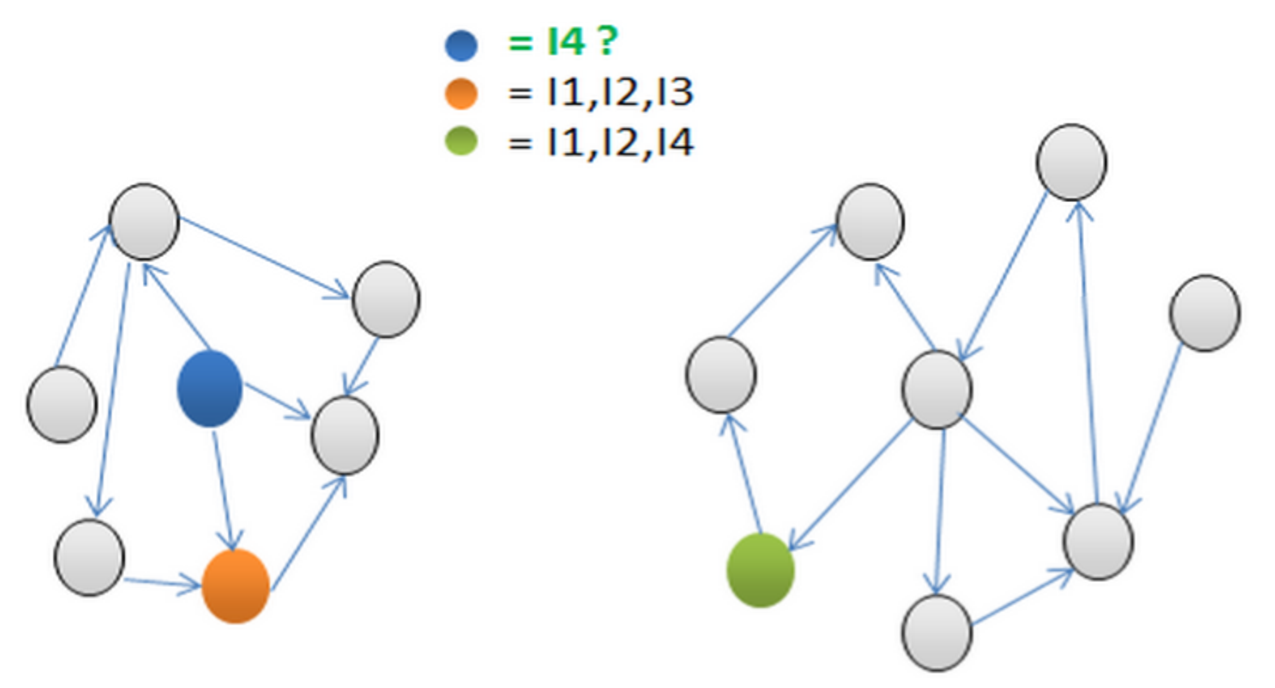
\includegraphics[width=0.4\textwidth]{fig1}
\caption{Example of trust network disjointedness. The trust network consists of two subgraphs, item I4 can not be recommended to the blue node user.}
\label{fig:motiv}
\end{figure}

Consider a recommender system with users $U = \{u_1, u_2, \dots, u_N \}$, and items $I = \{i_1, i_2, \dots, i_M \}$, where $N$ and $M$ are the users and items counts respectively. Each user $u \in U$ rated an item $i \in I$ with value $r_{u,i}$. We consider ratings with discrete values belonging to a finite set (e.g. $\{1,2,\dots,5\}$). Also, each user $u$ trusts a set of users $T(u) \subseteq U$. This trust information can be acquired explicitly (e.g. a user declares their trust), or implicitly (e.g. based on mutual activities). In this report, we consider a general trust values (e.g. not necessarily a binary). Given the trust information, we construct a directed trust network $T$, where nodes are the users, and weighted edges represent the trust information. Let the trust network $T$ consists of multiple subgraphs $T_1, T_2, \dots, T_d$ such that: $T = \cup_i^d~T_i$ and $\cap_i^d~T_i = \phi$. That is, the original trust network $T$ consists of disjoint trust networks, where trust information is not propagated across them. This \textit{typical} trust network structure reduces the recommendation coverage. Also, there is an inherent trade-off between the recommendation coverage and accuracy. For example, recommender systems can favor accuracy for coverage or vice versa, and such disjoint trust network will reduce coverage even more. Our \textit{goal} is to predict unknown item ratings $\widehat{r_{u,i}}$ to users in such a disjoint trust network, such that the coverage is maximized without significantly reducing the accuracy.


\section{TrusTem: recommender system in disjoint trust networks} \label{sec:solution}

\subsection{Graph-based Model}
As depicted in Figure~\ref{fig:motiv}, orange and blue nodes users have similar item preferences even though they belong to different subgraphs. One possible interpretation is that these two users have similar item preferences but they do not know each other. Therefore, if we can establish a link between these two users, not only we recommend trust but importantly we get rid of the coverage problem stated in the previous section. This link will work as the bridge between the two subgraphs.

\begin{figure}[tp]
\centering
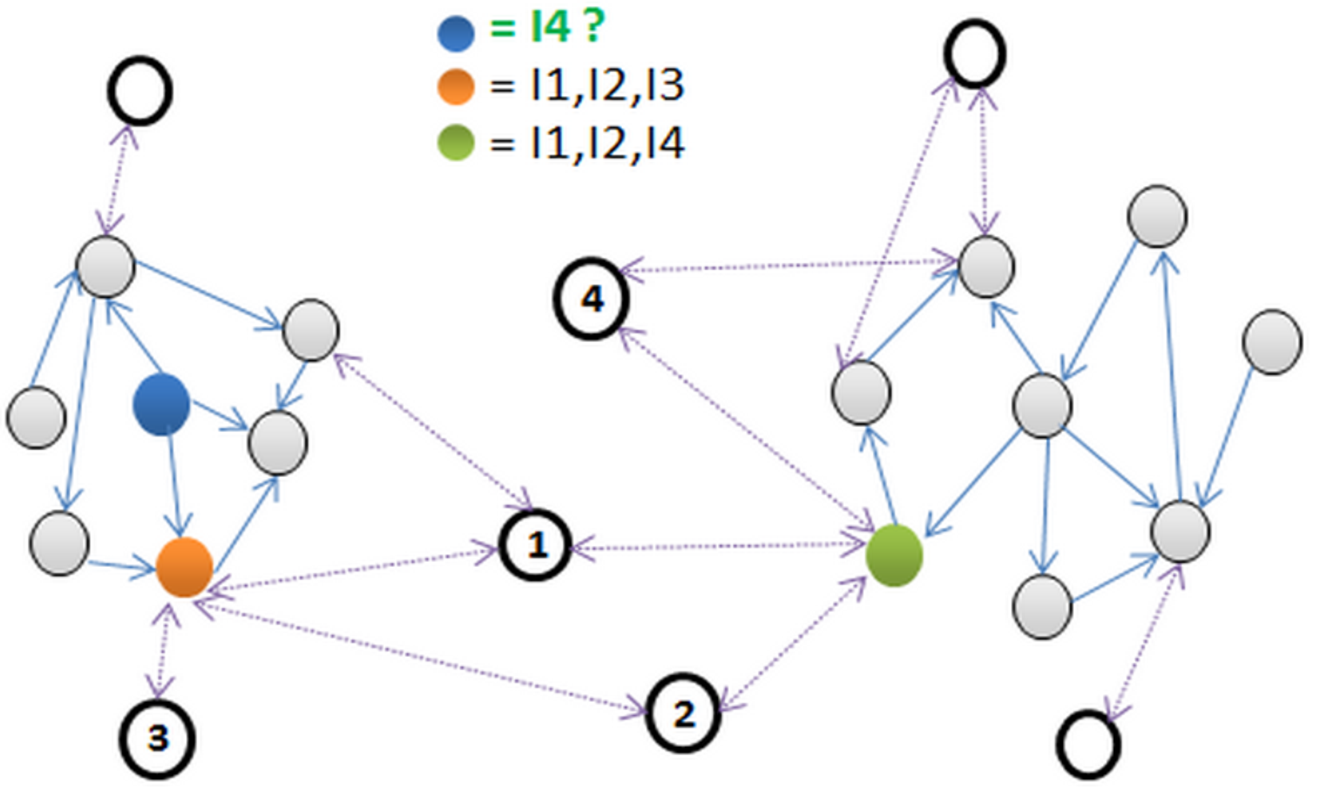
\includegraphics[width=0.4\textwidth]{fig2}
\caption{Bridging the disjoint trust networks by using items nodes between the subgraphs.}
\label{fig:link}
\end{figure}

To create such link between subgraphs, we introduce items as nodes within the original trust network. The network will no longer be trust network since there will be two different kinds of edges, user to user trust edges and user to item edges if the user rated the item. In Figure~\ref{fig:link}, it is evident that item I4 can be recommended to the blue node user, since it trusts the orange node user which is now linked to the green node user through the item nodes. 

\subsection{Matrix Representation and Factorization}
We address the problem of \textit{recommendation in disjoint trust networks} by considering a user-item and user-user matrices. This is different than some state-of-art algorithms, which adopted graph traversal techniques (such as TrustWalker~\cite{Jamali:2009}). We first build the two matrices using the user-item ratings and user trust information. Our model is based on merging both of the matrices as shown in Figure~\ref{fig:merge}. This indicates that trust information is considered as a rating as well.

\begin{figure}[tp]
\centering
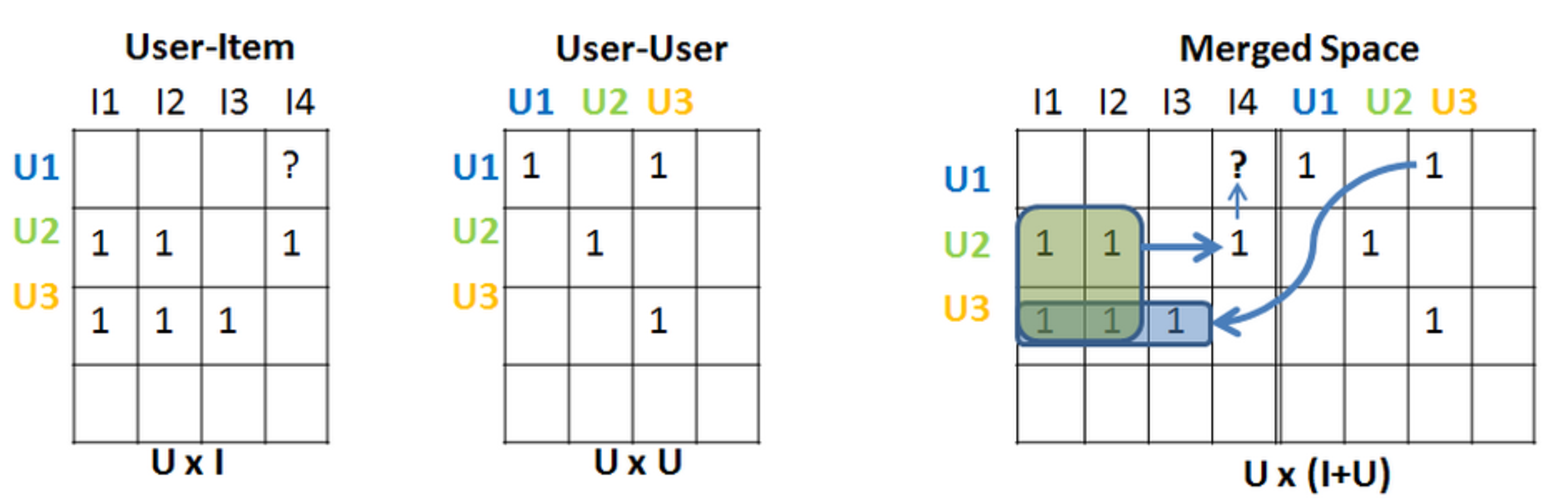
\includegraphics[width=0.6\textwidth]{fig3}
\caption{Merging the rating and trust domains in TrusTem.}
\label{fig:merge}
\end{figure}

We use matrix factorization technique to propagate trust and recommend items. Matrix factorization approximates the underlying relationship between users, items and trust in TrusTem. That is, given $K$ latent features (e.g. the underlying relationship), we can interpret matrix factorization results as follows. Each user  rates each item through these $K$ features. On the other hand, the same user may trust other users through the same $K$ features. For example, consider two users $u_1$ and $u_2$ and two items $i_1$ and $i_2$ and $K=2$. $u_1$ likes $i_1$ but not $i_2$, $u_2$ dislikes $i_1$ but likes $i_2$. Figure~\ref{fig:mf_example} shows the  merged matrix decomposition results.
 
\begin{figure}[tp]
\centering
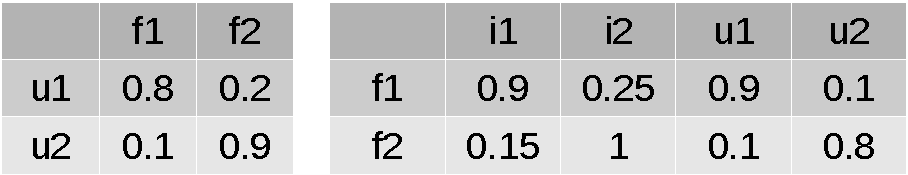
\includegraphics[width=0.4\textwidth]{example}
\caption{Illustration of matrix factorization interpretation in TrusTem.}
\label{fig:mf_example}
\end{figure}

\section{Evaluation}
We used the Epinions dataset, which includes $7,073$ users who rated a total of $139,738$ different items. In our experiments, we merged the ratings and trust matrices before running matrix factorization technique. We have set the latent features size to $K = 25$. In order to evaluate TrusTem, we use three performance metrics: (1) root mean squared-error (RMSE), (2) item coverage, (3) F-measure.
To calculate $RMSE$, we use the dataset $D$ that we already have ratings for.
\begin{equation}
RMSE = \sqrt{\frac{\sum_{(u,i)\in D}\left(r_{u,i} - \widehat{r_{u,i}} \right)^2}{|D|}}
\end{equation}
F-measure combines both accuracy and coverage in one numeric metric. We employ the same formulas as TrustWalker~\cite{Jamali:2009} to calculate F-measure. First, we convert the $RMSE$ to precision using the following equation:
\begin{equation}
precision = 1 - \frac{RMSE}{4}
\end{equation}
This represents the worst precision a recommender system can achieve, since the worst difference between actual and predicted ratings are $5-1 = 4$. Hence, F-measure can be calculated as follows:
\begin{equation}
Fmeasure = \frac{2\times precision \times coverage}{precision + coverage}
\end{equation}

These performance metrics applied on the user-item sub-matrix of the resultant matrix, since the user-user trust sub-matrix of the resultant matrix is usually considered as a secondary outcome of TrusTem.

We present our experiments results and comparison against other state-of-the-art algorithms. Table~\ref{tab:results} shows RMSE, coverage and F-measure of these models when used on the Epinions.com dataset. 

\begin{table}
\centering

\begin{tabular}{|l|l|l|l|}
\hline
\textbf{Method}            & \textbf{RMSE}    & \textbf{Coverage (\%)} & \textbf{F-Measure} \\ \hline \hline
TidalTrust~\cite{Golbeck:2005}  & $1.096$ & $84.9$        & $0.65$    \\ \hline
MoleTrust~\cite{Massa:2007}   & $1.093$ & $82.1$        & $0.608$   \\ \hline
TrustWalker~\cite{Jamali:2009} & $1.077$ & $95.4$        & $0.827$   \\ \hline
SocialMF~\cite{Jamali:2010}    & $1.085$ & NA            & NA        \\ \hline
TrusTem     & $1.172$ & $99.8$        & $0.828$   \\ \hline
\end{tabular}
\caption{Experimental results using Epinions.com dataset.}
\label{tab:results}
\end{table}

As shown in the table, TrusTem has better item coverage than the other models. TrustWalker model has one of the best item coverage which is around $95.4\%$ whereas our model has around $99.8\%$ coverage rate. However, we do not know the coverage rate of SocialMF which is a trust-based recommender system using matrix factorization technique. In SocialMF trust propagation happens through latent feature vector of every user and the latent feature of one user depends on their direct neighbor in the trust network, therefore, item coverage issue due to disjointedness will exist. Although TrusTem has improved item coverage rate compared to other methods but in terms of accuracy, it is $7\%$ and $8\%$ less than that of the SocialMF and TrustWalker methods respectively. However, TrusTem scores high F-measure compared to TidalTrust and MoleTrust. Also, it is as high as TrustWalker. It means that TrusTem almost does the same accuracy-coverage trade-off compared to TrustWalker.


\section{Conclusions}
In this report, we defined a new problem: in trust-based recommender systems, trust disjointedness is one of the reasons behind item coverage reduction. In order to address this problem we devised a new solution model, based on merging user-item rating and user-user trust domains. Then, we employ matrix factorization to recommend items. We discussed how trust in the merged matrix propagates to recommend items to users belong to different subgraphs. 
Experiments on real life dataset from Epinions.com demonstrate that TrusTem outperforms existing algorithms for item coverage and trades off rating accuracy to achieve that. Further, TrusTem exhibits better F-measure compared to these algorithms. This work suggests several directions for future work. Since items and users are represented in the same latent feature space, it implicitly describes the trust information based on several features. This gives us a notion that trust can be granularized into further details, which may improve the overall accuracy of the system. 


\bibliographystyle{IEEEtran}   
% refs.bib: should contain all references. One bib file that rules them all :)
\bibliography{./refs}    

\end{document}


